\documentclass[aspectratio=169]{beamer}

\usepackage[utf8]{inputenc}
\usepackage[english]{babel}
\usepackage[T1]{fontenc}
\usepackage{lmodern}
\usepackage{bbm}
\usepackage{listings}
\usepackage{multicol}
\usepackage{csquotes}
\usepackage{hyperref}
\usepackage{indentfirst}
\usepackage{amsthm}
\usepackage{amsfonts}
\usepackage{amsmath}
\usepackage{amssymb}
\usepackage{mathtools}
\usepackage{tikz}
\usepackage{xcolor}
\usepackage{array}
\usepackage{bookmark}
\usepackage{booktabs}

\newcommand{\id}[1]{\ensuremath{\mathit{#1}}}
\newcommand{\kw}[1]{\ensuremath{\mathtt{#1}}}
\newcommand{\Let}{\kw{let}}
\newcommand{\In}{\kw{in}}
\newcommand{\If}{\kw{if}}
\newcommand{\Then}{\kw{then}}
\newcommand{\Else}{\kw{else}}
\newcommand{\Filter}{\kw{filter}}
\newcommand{\Or}{\kw{or}}
\newcommand{\Groupby}{\kw{groupby}}
\newcommand{\Partition}{\kw{partition}}
\newcommand{\Scatter}{\kw{scatter}}
\newcommand{\Hist}{\kw{hist}}
\newcommand{\Map}{\kw{map}}
\newcommand{\Sum}{\kw{sum}}
\newcommand{\Mod}{\kw{mod}}
\newcommand{\Fst}{\kw{fst}}
\newcommand{\Snd}{\kw{snd}}
\newcommand{\Presum}{\kw{presum}}
\newcommand{\True}{\kw{true}}
\newcommand{\False}{\kw{false}}
\newcommand{\Sort}{\kw{sort}}
\newcommand{\Segor}{\kw{segor}}
\newcommand{\Hash}{\kw{hash}}
\newcommand{\Random}{\kw{random}}
\newcommand{\Iota}{\kw{iota}}
\newcommand{\Unzip}{\kw{unzip}}
\newcommand{\Unit}{\mathbf{unit}}
\newcommand{\Int}{\mathbf{int}}
\newcommand{\Bool}{\mathbf{bool}}
\newcommand{\Def}{\kw{def}}
\newcommand{\While}{\kw{while}}
\newcommand{\Do}{\kw{do}}
\newcommand{\Rep}{\kw{rep}}
\newcommand{\Zip}{\kw{zip}}

\usetikzlibrary{automata, positioning, arrows}

\graphicspath{ {./figures/} }

\definecolor{palepurple}{rgb}{0.7647,0.69411,0.88235}
\definecolor{palepurple}{rgb}{0.7647,0.69411,0.88235}
\definecolor{midviolet}{rgb}{0.6,0.4,0.8}

\newcolumntype{M}[2]{>{\centering\arraybackslash}m{#1}<{\rule{0pt}{#2}}}
\newcommand{\darkpalepurple}{palepurple!70!black}
\definecolor{paleyellow}{rgb}{1.0,1.0,0.7725}
\setbeamercolor{background canvas}{bg=paleyellow}

\usetheme{default}
\usecolortheme{wolverine}
\setbeamercolor*{palette primary}{bg=palepurple}
\setbeamercolor*{palette quaternary}{bg=palepurple}
\setbeamercolor{structure}{fg=palepurple}
\setbeamertemplate{navigation symbols}{\insertframenumber/\inserttotalframenumber}
\setbeamertemplate{blocks}[rounded][shadow]
\setbeamercolor{frametitle}{bg=midviolet,fg=black}
\setbeamercolor{block title}{bg=structure, fg=black}
\setbeamercolor{block body}{bg=structure, fg=black}
\setbeamercolor{block title alerted}{bg=structure, fg=black}
\setbeamercolor{block body alerted}{bg=structure, fg=black}
\setbeamercolor{block title example}{bg=structure, fg=black}
\setbeamercolor{block body example}{bg=structure, fg=black}
\setbeamercolor{frametitle}{bg=palepurple,fg=black}


\setbeamertemplate{itemize item}{\scriptsize$\blacksquare$}
\setbeamertemplate{itemize subitem}{\scriptsize$\blacksquare$}
\setbeamertemplate{itemize subsubitem}{\scriptsize$\blacksquare$}

\title[Programming]{Programming}
\author{\textbf{William Henrich Due} \inst{1}}
\institute[shortinst]{\inst{1} Department of Computer Science}
\date{September 12th, 2025}

\begin{document}

\begin{frame}
  \begin{center}
    \titlepage
    \vfill
  \end{center}
\end{frame}

\begin{frame}\frametitle{Intended Learning Outcomes}
  \begin{itemize}
    \item Write a simple program as a nondetermistic finite-state automaton (NFA).
    \item Write a simple program as a determistic finite-state automaton (DFA).
    \item The ability to differentiate between a NFA and a DFA.
  \end{itemize}
\end{frame}

\begin{frame}\frametitle{Programming Languages}
  \begin{center}
    What Programming Languages do you know?
  \end{center}
\end{frame}

\begin{frame}\frametitle{NFA}
  \begin{itemize}
    \item An alphabet that is a finite set of symbols e.g.
    \begin{itemize}
      \item English Alphabet.
      \item Hindu--Arabic numerals.
      \item Morse code symbols.
    \end{itemize}

    \item A finite set of states $\vcenter{
      \hbox{
        
\begin{tikzpicture}[baseline]
          \node[state] (s) {$$};
        \end{tikzpicture}
      }
    }$

    \item Transitions between states labelled by symbols or $\varepsilon$.
    
    $\vcenter{
      \hbox{
        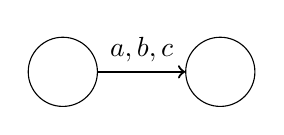
\begin{tikzpicture}[baseline]
          \node[state] (s) at (0,0) {$$};
          \node[state] (sp) at (2,0) {$$};
          \draw[->, thick] (s) -- node[above] {$a,b,c$} (sp);
        \end{tikzpicture}
      }
    }$ $\vcenter{
      \hbox{
        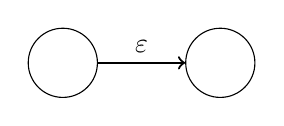
\begin{tikzpicture}[baseline]
          \node[state] (s) at (0,0) {$$};
          \node[state] (sp) at (2,0) {$$};
          \draw[->, thick] (s) -- node[above] {$\varepsilon$} (sp);
        \end{tikzpicture}
      }
    }$

    \item A single initial state.
    $\vcenter{
      \hbox{
        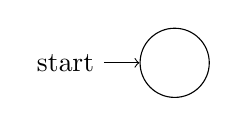
\begin{tikzpicture}[baseline]
          \node[state, initial] (s) {$$};
        \end{tikzpicture}
      }
    }$
    \item Zero or more accepting states.
    $\vcenter{
      \hbox{
        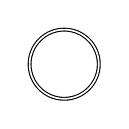
\begin{tikzpicture}[baseline]
          \node[state, accepting] (s) {$$};
        \end{tikzpicture}
      }
    }$
  \end{itemize}
\end{frame}

\begin{frame}\frametitle{NFA Simulation}
  \begin{center}
    \begin{tikzpicture}[shorten >=1pt, node distance=2.6cm, on grid, auto, >=stealth', baseline]
      % Step overlays for states
      % Initial state
      \only<1,2-4,6-7,9->{\tikzset{stateq0/.style={state, initial, fill=none}}}
      \only<2,5,8>{\tikzset{stateq0/.style={state, initial, fill=palepurple, ultra thick}}}

      % Accepting state (top)
      \only<1-2,4->{\tikzset{stateq1/.style={state, accepting, fill=none}}}
      \only<3>{\tikzset{stateq1/.style={state, accepting, fill=palepurple, ultra thick}}}
      
      % Intermediate state (middle)
      \only<1-8,10->{\tikzset{stateq2/.style={state, fill=none}}}
      \only<9>{\tikzset{stateq2/.style={state, fill=palepurple, ultra thick}}}
      
      % Accepting state (right)
      \only<1-9,11->{\tikzset{stateq3/.style={state, accepting, fill=none}}}
      \only<10>{\tikzset{stateq3/.style={state, accepting, fill=palepurple, ultra thick}}}
      
      % Accepting state (bottom, epsilon)
      \only<1-5,7->{\tikzset{stateq4/.style={state, accepting, fill=none}}}
      \only<6>{\tikzset{stateq4/.style={state, accepting, fill=palepurple, ultra thick}}}
      
      % Edge overlays
      \only<1-2,4->{\tikzset{edgea1/.style={}}}
      \only<3>{\tikzset{edgea1/.style={\darkpalepurple, line width=1.5pt}}}
      
      \only<1-8,9->{\tikzset{edgea2/.style={}}}
      \only<9>{\tikzset{edgea2/.style={\darkpalepurple, line width=1.5pt}}}
      
      \only<1-9,11->{\tikzset{edgea3/.style={}}}
      \only<10>{\tikzset{edgea3/.style={\darkpalepurple, line width=1.5pt}}}
      
      \only<1-5,7->{\tikzset{edgeeps/.style={}}}
      \only<6>{\tikzset{edgeeps/.style={\darkpalepurple, line width=1.5pt}}}
      
      % Nodes
      \node[stateq0] (q0) {};
      \node[stateq1] (q1) [above right=2cm and 2cm of q0] {};
      \node[stateq2] (q2) [right=of q0] {};
      \node[stateq3] (q3) [right=of q2] {};
      \node[stateq4] (q4) [below right=2cm and 2cm of q0] {};
      
      % Edges
      \draw[->,edgea1] (q0) -- node[above left] {$a,b$} (q1);
      \draw[->,edgea2] (q0) -- node[above] {$a$} (q2);
      \draw[->,edgea3] (q2) -- node[above] {$b$} (q3);
      \draw[->,edgeeps] (q0) -- node[left] {$\varepsilon$} (q4);
    \end{tikzpicture}

    \vspace{10pt}
    % Input string animation
    \only<1-2,4-8>{\Huge\bfseries\color{gray}ab}
    \only<3,9>{\Huge\bfseries\color{black}a\color{gray}b}
    \only<10>{\Huge\bfseries\color{gray}a\color{black}b}
    \only<11>{\Huge\bfseries\color{black}ab}
    \vspace{10pt}
    % Acceptance message
    \only<11>{\Large\bfseries\color{black}Accepted!}
  \end{center}
\end{frame}

\begin{frame}\frametitle{Your turn}
  \begin{center}
    Create a NFA that determines if a non-negative integer is even.
  \end{center}
\end{frame}

\begin{frame}\frametitle{DFA}
  \begin{itemize}
    \item Subset of NFAs.

    \item No $\varepsilon$ transitions allowed.
    
    $\vcenter{
      \hbox{
        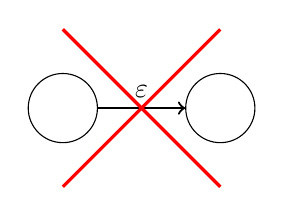
\begin{tikzpicture}[baseline]
          % Original states and transition
          \node[state] (s) at (0,0) {};
          \node[state] (sp) at (2,0) {};
          \draw[->, thick] (s) -- node[above] {$\varepsilon$} (sp);
    
        % Big red X over the diagram
        \draw[red, very thick] (-0.0,1.0) -- (2.0,-1.0);
        \draw[red, very thick] (-0.0,-1.0) -- (2.0,1.0);
      \end{tikzpicture}
    }
    }$

    \item No state may have more than one outgoing transition per symbol.
    
    $\vcenter{
      \hbox{
        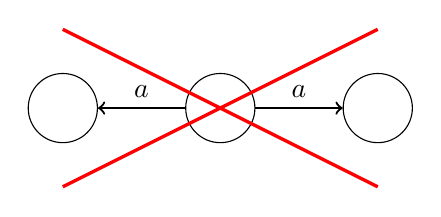
\begin{tikzpicture}[baseline]
          \node[state] (s) at (0,0) {$$};
          \node[state] (sp) at (2,0) {$$};
          \node[state] (si) at (-2,0) {$$};
          \draw[->, thick] (s) -- node[above] {$a$} (sp);
          \draw[->, thick] (s) -- node[above] {$a$} (si);

          \draw[red, very thick] (-2.0,1.0) -- (2.0,-1.0);
          \draw[red, very thick] (-2.0,-1.0) -- (2.0,1.0);
        \end{tikzpicture}
      }
    }$
    \item Why do this?
  \end{itemize}
\end{frame}


\begin{frame}\frametitle{Your turn}
  \begin{center}
    Create a DFA that determines if a non-negative integer is even.
  \end{center}
\end{frame}

\begin{frame}\frametitle{We are done}
  \begin{center}
    We are done.
  \end{center}
\end{frame}

\end{document}